\subsection{Gruppestruktur}
Vi har allerede definert elliptiske kurver som en varietet. I denne seksjonen skal vi vise at den også danner en abelsk gruppe under en spesifikk operasjon og noen viktige konsekvenser av det.

Aller først må vi introdusere noen flere geometriske begreper så vi kan definere selve operasjonen.

\begin{definisjon}
La $V/K$ være en varietet i det projektive rommet. Vi ser at $V/K$ er en \textbf{linje} dersom idealet er generert av et polynom av grad én, altså $f(X,Y,Z) = aX + bY + cZ$ for $a,b,c \in K$.
\end{definisjon}

\begin{proposisjon}
To unike punkter, $P_1$, $P_2$ i det projektive planet danner en unik linje. 
\begin{proof}
La $P_1 = [x,y,z]$ og $P_2 = [x', y', z']$. En linje $L$ gjennom $P_1$ og $P_2$ der $f(X,Y,Z)$ er polynomet som genererer idealet. Da vil naturligvis $f(P_1) = f(P_2) = $, altså har vi $ax + by + cz = 0$ og $ax' + by' + cz' = 0$. Med vanlig lineær algebra kan vi skrive dette som 
\begin{equation*}
\begin{bmatrix}
x & y & z \\
x' & y' & z
\end{bmatrix}
\begin{bmatrix}
a \\
b \\
c
\end{bmatrix}
= 
\begin{bmatrix}
0 \\
0
\end{bmatrix}
\end{equation*}
Siden $P_1$ og $P_2$ er ulike vil de to radene i den første matrisen være lineært uavhengige - altså har vi at $a,b,c$ er en unik løsning opp til skalarmultiplikasjon. Men siden vi jobber i det projektive planet vil $(a,b,c)$ og $(\lambda a, \lambda b, \lambda c)$ være samme punkt, så $(a,b,c)$ danner en unik linje $ax + by, cz$ i $\Projective^2$. 
\textbf{TODO: Bevis dette annerledes! - dette er sannsynligvis feil}
\end{proof}
\end{proposisjon}

\begin{definisjon}
La $V_1/K$ og $V_2/K$ være to varieteter. Vi sier at $P$ er et \textbf{skjæringspunkt} dersom $P \in V_1 \cap V_2$, altså ligger punktet i begge varietetene. Vi kommer i denne teksten til å skrive $V_1 \circ V_2$ for å betegne mengden av alle skjæringspunkter mellom varietetene.
\end{definisjon}

Multiplisiteten til et skjæringspunkt er en relativt komplisert affære, og kunne fint fått sin egen seksjon i denne teksten. Men siden vi ikke kommer til å bruke det til noe annet enn for å bevise at en elliptisk kurve er en gruppe benytter vi oss av et av resultatene fra en mer generell beskrivelse. Her er blant annet kravet at $P$ er ikke-singulær, men siden $E$ er en elliptisk kurve får vi dette gratis. For mer informasjon om multiplisitet til skjæringspunkt kan du lese \cite[3.3]{fulton}
\begin{definisjon}
La $P$ være et skjæringspunkt mellom en elliptisk kurve $E$ og en varietet $V$. Vi sier at \textbf{multiplisiteten} til punktet er $ord_p^{E}(V)$.
\end{definisjon}

\begin{teorem}
\textbf{Bézouts teorem} La $E/K$ være en elliptisk kurve, og $L$ en linje - begge i det projektive planet. Da vil Linjen og kurven skjære hverandre i nøyaktig tre punkter dersom vi teller multiplisiteten til punktene. 
\cite[5.3]{fulton}
%La $V_1/K$ og $V_2/K$ være to varieteter i det projektive rommet henholdsvis definert av de irredusible polynomene $f_1$ og $f_2$ av dimensjoner $n_1$ og $n_2$. Da vil de to varietetene skjære hverandre i nøyaktig $n = n_1 * n_2$ punkter hvis vi teller multiplisitet til punktene. 
\end{teorem}
Merk, teoremet er mye mer generelt enn dette, men til våre formål er det dette som er essensielt.

\begin{figure}[h!]
\centering
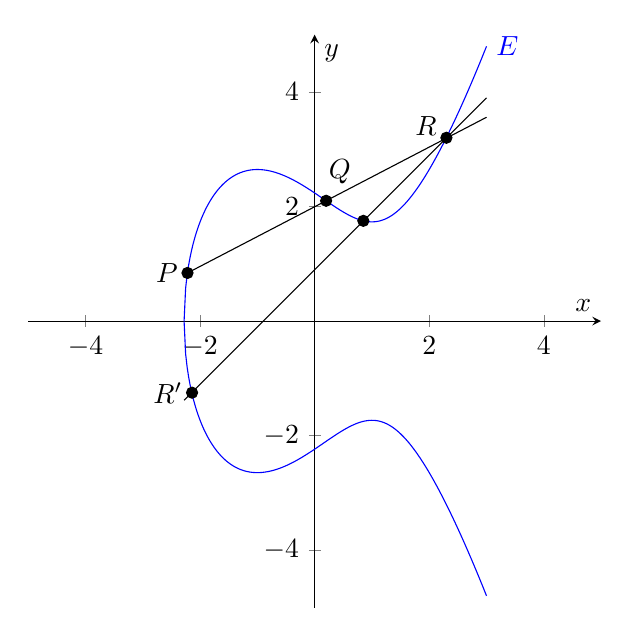
\begin{tikzpicture}

\begin{axis}[
xmin=-5,
xmax=5,
ymin=-5,
ymax=5,
xlabel={$x$},
ylabel={$y$},
scale only axis,
axis lines = middle,
domain=-2.2790178:3,
samples=201,
clip=false,
axis equal image=true
]
\addplot[blue] {sqrt(x^3-3*x+5)} node[right] {$E$};
\addplot[blue] {-sqrt(x^3-3*x+5)};
\addplot[black] { 4.83 / 2.42 + 1.26*x / 2.42};
\addplot[black] { 1.3 / 1.45 + x};


\draw[fill=black] (axis cs: -2.22, 0.84) circle (2pt) node [left] {$P$};
\draw[fill=black] (axis cs:  0.2, 2.1) circle (2pt);
\draw[color=black] (axis cs: 0.8, 2.6) node[left]{$Q$};
\draw[fill=black] (axis cs: 2.3, 3.2) circle (2pt);
\draw[color=black] (axis cs: 2.3, 3.4) node[left]{$R$};
\draw[fill=black] (axis cs: 0.85, 1.75) circle (2pt);
\draw[color=blue] (axis cs: 0.80, 1.6) node[left]{$\OO$};
\draw[fill=black] (axis cs: -2.14, -1.25) circle (2pt) node [left] {$R'$};
%\draw[color=black] (axis cs: -1.5, 2.7) node [left] {$P$};
\end{axis}
\end{tikzpicture}
\caption{Addisjon med baseelement $\OO$}
\end{figure}

\textbf{Skjæringspunkter}. La $C/K$ være en kurve som også er en varietet (tenk elliptisk kurve). Dersom vi tar to vilkårlige punkter $P, Q \in C$ får vi en unik linje, $L$, gjennom disse to punktene. Fra Bézouts teorem vet vi at denne linjen skjærer kurven i tre punkter. $L \circ C = \{P, Q, R \}$ for en $R \in C$. I spesialtilfellet der $P = Q$ setter vi linjen til å være tangentlinjen til $P$. Vi definerer nå avbildingen $\phi: C \times C \rightarrow C$ $(P, Q) \mapsto R$. Legg merke til at uansett hvilke to punkter du tar fra mengden av skjæringspunkter vil du alltid få den tredje. Dersom $L \circ C = \{P, Q, R\}$ vil $\phi(P, Q) = R$ og $\phi(P, R) = Q$ og $\phi(Q, R) = P$.

\begin{teorem}
En elliptisk kurve $E/K$ sammen med et baseelement $\OO \in E$ danner en abelsk gruppe under operasjonen $P + Q = \phi(\OO, \phi(P, Q))$, der $\phi$ er definert som over.

\begin{proof}
Vi må vise at $E$ er en gruppe og at den er abelsk, altså at den er assosiativ, har identitetselement, at alle punkter har en invers, og at den er kommutativ. La $P, Q, R \in E$, med $\OO$ som baseelement.
\begin{description}
\item[Assosiativitet] Skal vise at $(P + Q)+ R = P + (Q + R)$. La oss først definere noen punkter: $\phi(P,Q) = S'$, $\phi(\OO, S') = S$, $\phi(S, R) = T'$, $\phi(Q, R) = U'$, $\phi(\OO, U') = U$, $\phi(P, U) = T''$. Da har vi $(P + Q) + R) = \phi(\OO, T')$ og $P + (Q + R) = \phi(\OO, T'')$. Altså er det nok å vise at $T' = T''$.

Fra punktene over kan vi lage linjer som går gjennom punktene: $L_1: \{P, Q, S'\}$, $M_1: \{\OO, S', S\}$, $L_2: \{S, R, T' \}$, $M_2: \{ Q, R, U'\}$, $L_3: \{\OO, U', U \}$, $M_3: \{P, U, T''\}$ (Her er f.eks. $L_1$ linjen som går gjennom $P, Q, S'$ - det er der den skjærer $E$).

Vi kan nå sette sammen disse linjene ved enkel multiplikasjon. Husk at graden til hver linje er 1, så $L = L_1 * L_2 * L_3$ har grad 3 og er en kubisk kurve (ikke nødvendigvis irredusibel). Tilsvarende er $M = M_1 * M_2 * M_3$. 

La oss nå se på skjæringspunktene mellom disse linjene og kurven $E$. $E \circ L = \{P, Q, S', S, R, \OO, U', U, T' \}$, mens $E \circ M = \{\OO, S', S, Q, R, U', P, U, T'' \}$. Legg merke til at den eneste forskjellen er $T'$ og $T''$.

La oss nå lage en linje gjennom $T'$ som ikke går gjennom $T''$, Da har vi $N: \{T', W, W'\}$ for punkter $W, W' \in E$. Siden ingen av disse er i $M$ kan vi se på skjæringen mellom $N*M$ og $E$. $N*M \circ E = \{\OO, S',$ $ S, $ $ Q, $ $R, $ $U',$ $ P, $ $U, $ $T'',$ $ T',$ $ W,$ $ W'\}$ $ = L \circ E \cup \{T'', W, W' \}$, altså finnes det en linje mellom $T'', W$ og $ W'$. Denne linjen må nødvendigvis være lik $N$ da den deler to punkter, så $T' = T''$ og vi har vist at operasjonen ar assosiativ. \cite[5.6.4]{fulton}

\item[Identitet] La $\phi(\OO, P) =R $, da har vi $P + \OO = \phi(\OO, \phi(P, \OO)) = \phi(\OO, R) = P$, samtidig er $\OO + P = \phi(\OO, \phi(P, \OO)) = \phi(\OO, R) = P$
\item[Invers] La $\phi(\OO, P) = R$, da har vi at $(P + \OO) + R = \OO + P + R = \OO + \OO = \phi(\OO, \phi(\OO, \OO))$. Annta $\{\OO, \OO, Q \}$ ligger på samme linje ($\phi(\OO, \OO) = Q$), da har vi $\phi(\OO, \phi(\OO, \OO)) = \phi(\OO, Q) = \OO$.
\item[Kommutativitet] Siden $\phi(P, Q) = \phi(Q,P)$ da dette bare er det tredje punktet på linjen har vi $P + Q = \phi(\OO, \phi(P, Q)) = \phi(\OO, \phi(Q,P)) = Q + P$
\end{description}
\end{proof}
\end{teorem}

Nå som vi vet at en elliptisk kurve danner en abelsk gruppe for et vilkårlig baseelement kan vi bestemme oss for et spesifikt. Det er vanlig å bruke punktet $[0,1,0]$ som baseelement/punkt i uendeligheten. Så videre i denne teksten anntar vi at $\OO = [0,1,0]$ da det forenkler en del regning. Legg merke til hvordan $\phi((x,y), \OO) = (x, -y)$ linjen mellom et punkt og $\OO$ blir den vertikale linjen.

Dette fører til at dersom $P = (x,y)$ vil $-P = \phi(P, \OO) = (x, -y)$.

Vi kommer til å bruke notasjonen $E(K)$ for å referere til de $K$-rasjonale punktene i $E$.

%$O = [0,1,0]$

%\subsection{Weierstrass form}
%\subsection{Invarianter}
%\subsection{Torsionundergrupper}
%Hva er dette, hvordan fungerer de.
%Hvorfor har vi $E[l]$ der $l$ deler $[E]$

%Hva er en supersingulær elliptisk kurve, finnes det alltid en slik?